\section{ROC --- Rate Of Change indicator}
\label{sec:1ROC}
Rate Of Change is an indicator which measures the percentage change between the latest price and closing price of $k$ periods before. The method of calculating the value of the ROC, for a given point in time, represent formulas \ref{wzorroc_1} and \ref{wzorroc_2}.
\begin{equation}
ROC(\text{now}) = \frac{\text{Current close price} - \text{Close price} k \text{ periods before}}{\text{Close price } k \text{ periods before}}\\
\label{wzorroc_1}
\end{equation}
\begin{equation}
ROC(i) = \frac{C(i,4) - C(i-k,4)}{C(i-k,4)}
\label{wzorroc_2}
\end{equation}

\noindent The basic properties of the ROC curve are:
\begin{itemize}
\item it shows how the observed market price during the period changed,
\item when the oscillator value is below zero, then the current price is higher than one from $k$-candles ago; analogically, when the oscillator is above zero, it means that the current price is lower than the price from $k$-candles ago,
\item increasing indicator line shows that the differences between the current prices and ones from $k$-time ago are increasing, decreasing says, that this differences decrease,
\item if the stock prices rise it can be expected that the oscillator line will behave in the same way; if the prices decrease the oscillator line should decrease.
\end{itemize}
The most important property of the described indicator, used while implementing  the strategy, is that it indicates the moments in which transactions should be made. When the value of the indicator crosses the zero level from below, it is assumed that this is a good time to buy, if it crosses the zero level from above, this is the good time to sale. This is shown in Figure \ref{kupsprzroc}.\\
\begin{figure}[h!]
\centering
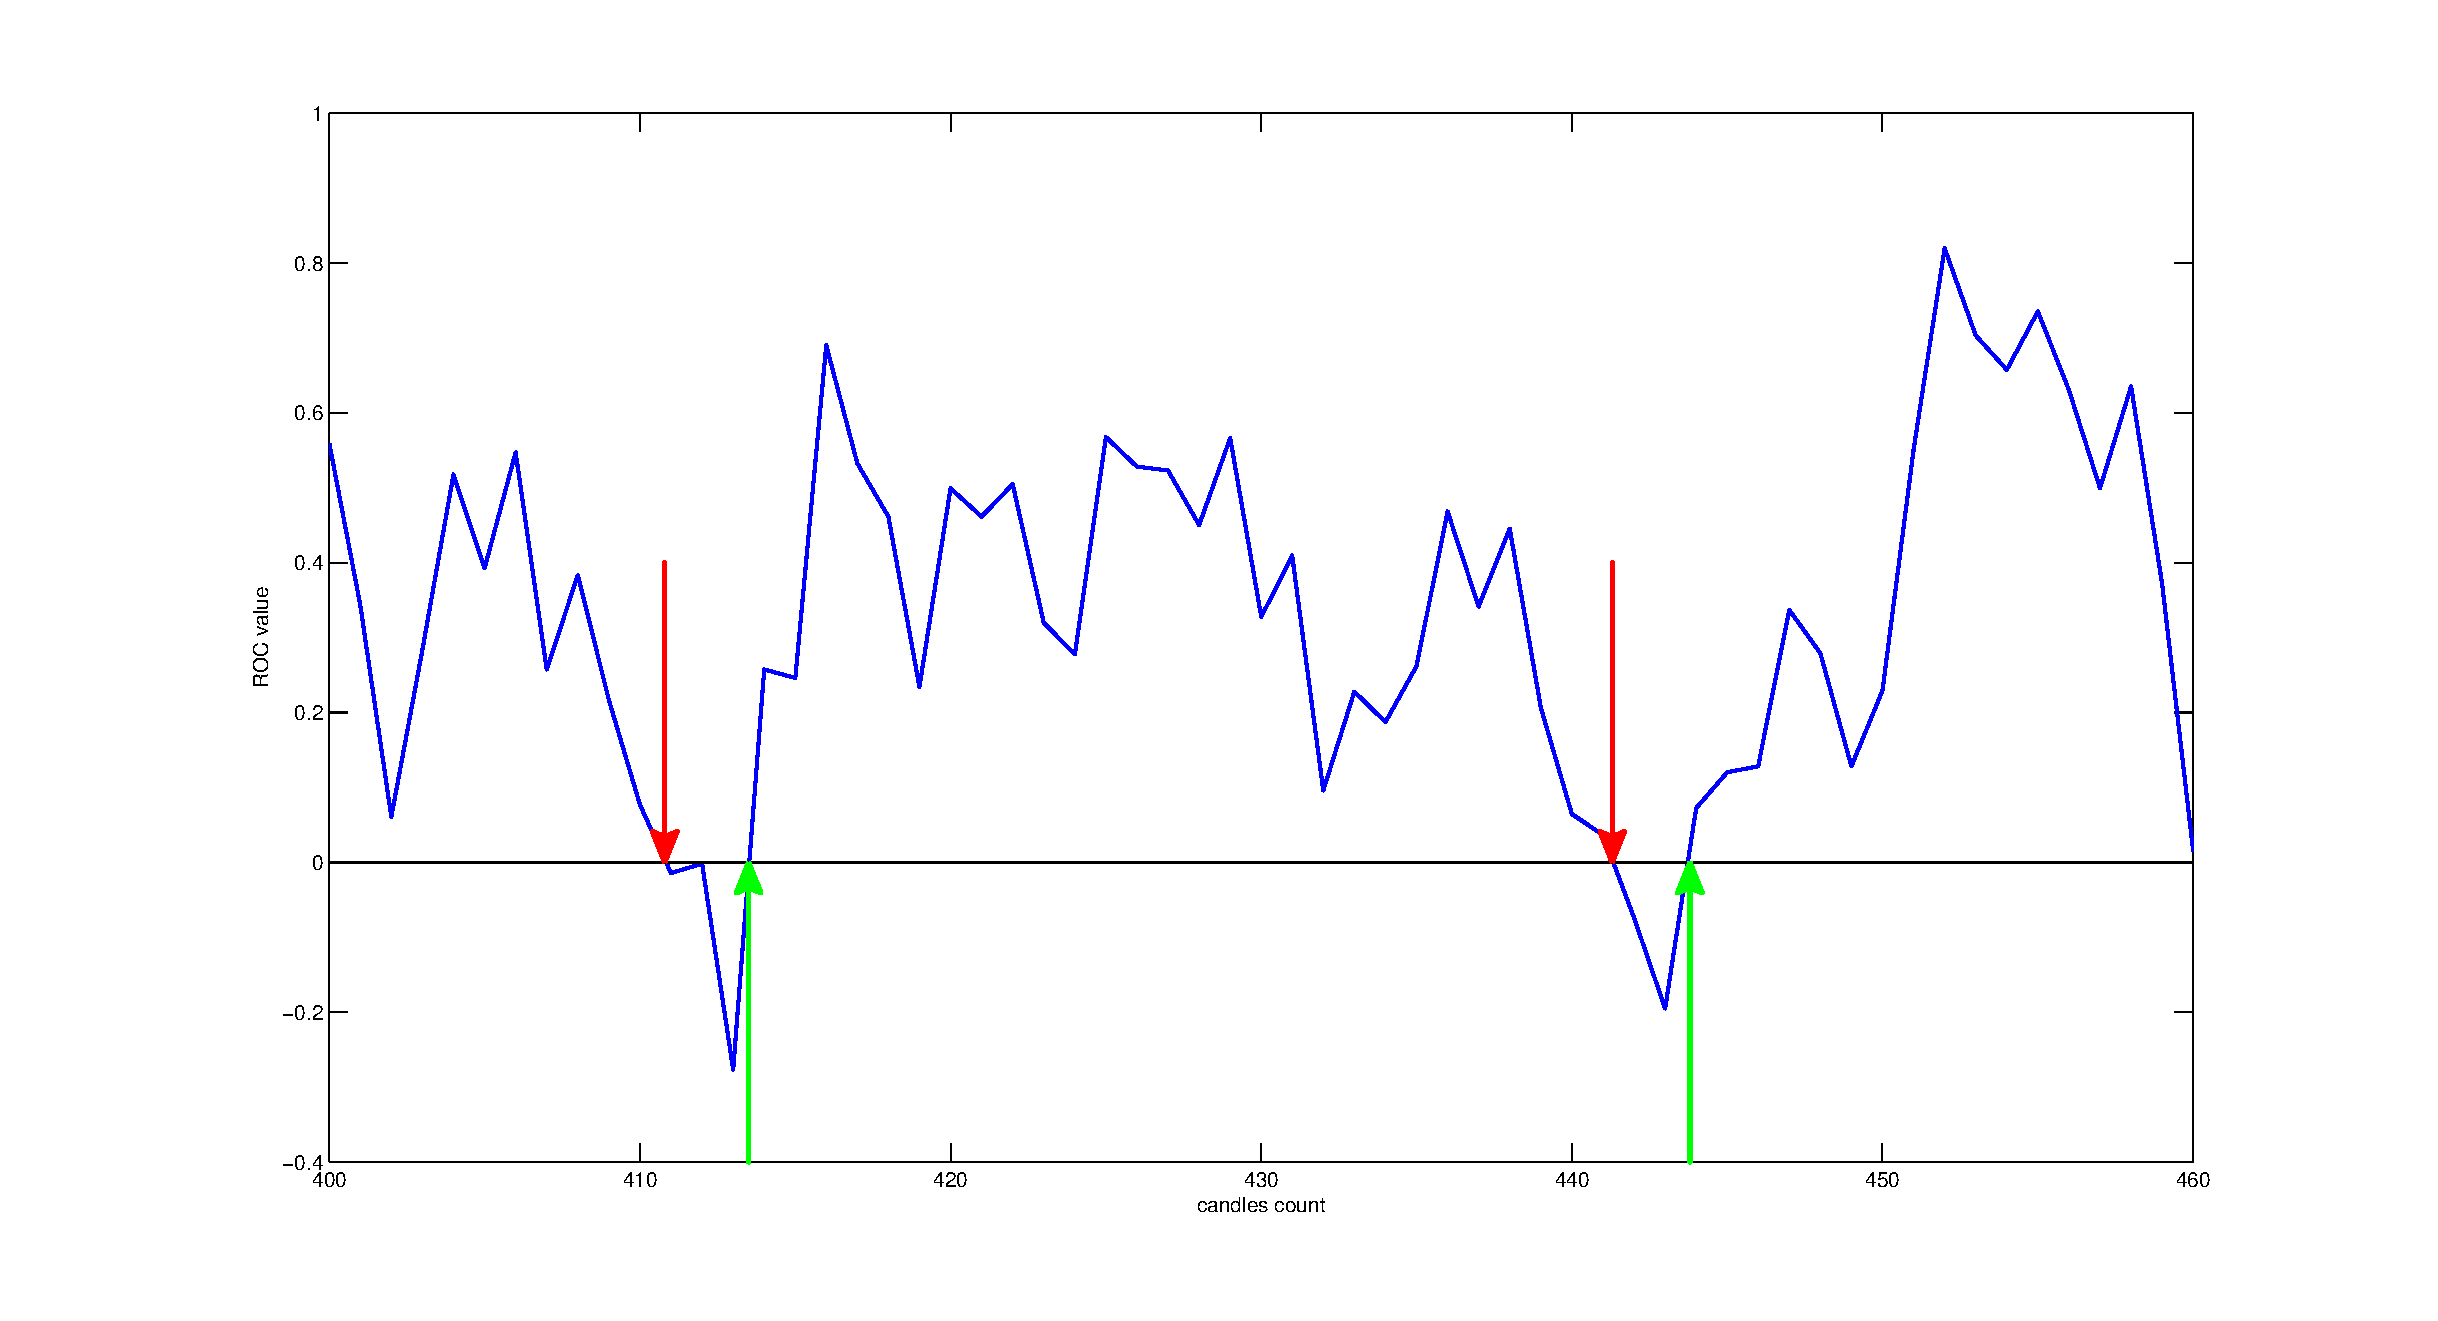
\includegraphics[width = \textwidth]{BuySell.eps}
\caption{Part of the sample ROC curve with buying signals --- green arrows --- and selling signals --- red arrows}
\label{kupsprzroc}
\end{figure}
\FloatBarrier

\noindent The following listing shows the strategy implemented in MATLAB.
\begin{scriptsize}
\begin{lstlisting}
pocz = k+2;	
kon = size(C,1)-1;
iL = 0; % exceeding 0 to top - buy(L)
iS = 0; % exceeding 0 to bottom - sell(S)
sumR = zeros(1,size(C,1));
R = zeros(1,size(C,1));
ROC_vec = zeros(1,kon-k+1);
ROC_vec(pocz-1) = ((C(pocz-1,4) - C(pocz-1-k,4))/C(pocz-1-k,4))*100;

recordReturn = 0;  % record profit
recordDrawdown = 0;  % record drawdown
LastPos = 0;    % variable used to store the value of the opening of the last position

for i=pocz:kon
   ROC_vec(i) = ((C(i,4) - C(i-k,4))/C(i-k,4))*100;  % calculating the ROC curve
   if ROC_vec(i)*ROC_vec(i-1)<=0   % the intersection of the ROC curve with zero
       if ROC_vec(i-1)<ROC_vec(i)  % a condition of purchase
           if iL+iS>0
               R(i) = -C(i+1,4)+LastPos-spread;   % closing S
           end
           LastPos = C(i+1,1);   % open L
           iL = iL + 1;
       elseif ROC_vec(i-1)>ROC_vec(i)  % a condition of sale
           if iL+iS>0
               R(i) = C(i+1,4)-LastPos-spread;  % closing L
           end
           LastPos = C(i+1,1);   % open S
           iS = iS + 1;
       end
   end
   sumR(i) = sum(R(pocz:i));
    if sumR(i)>recordReturn
       recordReturn=sumR(i);
   end
  
   if sumR(i)-recordReturn<recordDrawdown
       recordDrawdown=sumR(i)-recordReturn; 
   end

end

Calmar=-sumR(kon)/recordDrawdown;
profit = sumR(kon);

end
\end{lstlisting}
\end{scriptsize}


Based on collected information on the $ROC$ ratio a simple investment strategy, based on the rule: if the $ROC$ line intersects the zero level from below, it opens a long position ($L$) and closed a short position ($S$) which has been previously opened, was created. When $ROC$ line intersects zero level from above it will open a short position and close a long one. Tests were carried out on $EURJPY$ currency pair (time series shown in Figure \ref{rysunek2roc}).\\

\begin{figure}[h!]
\centering
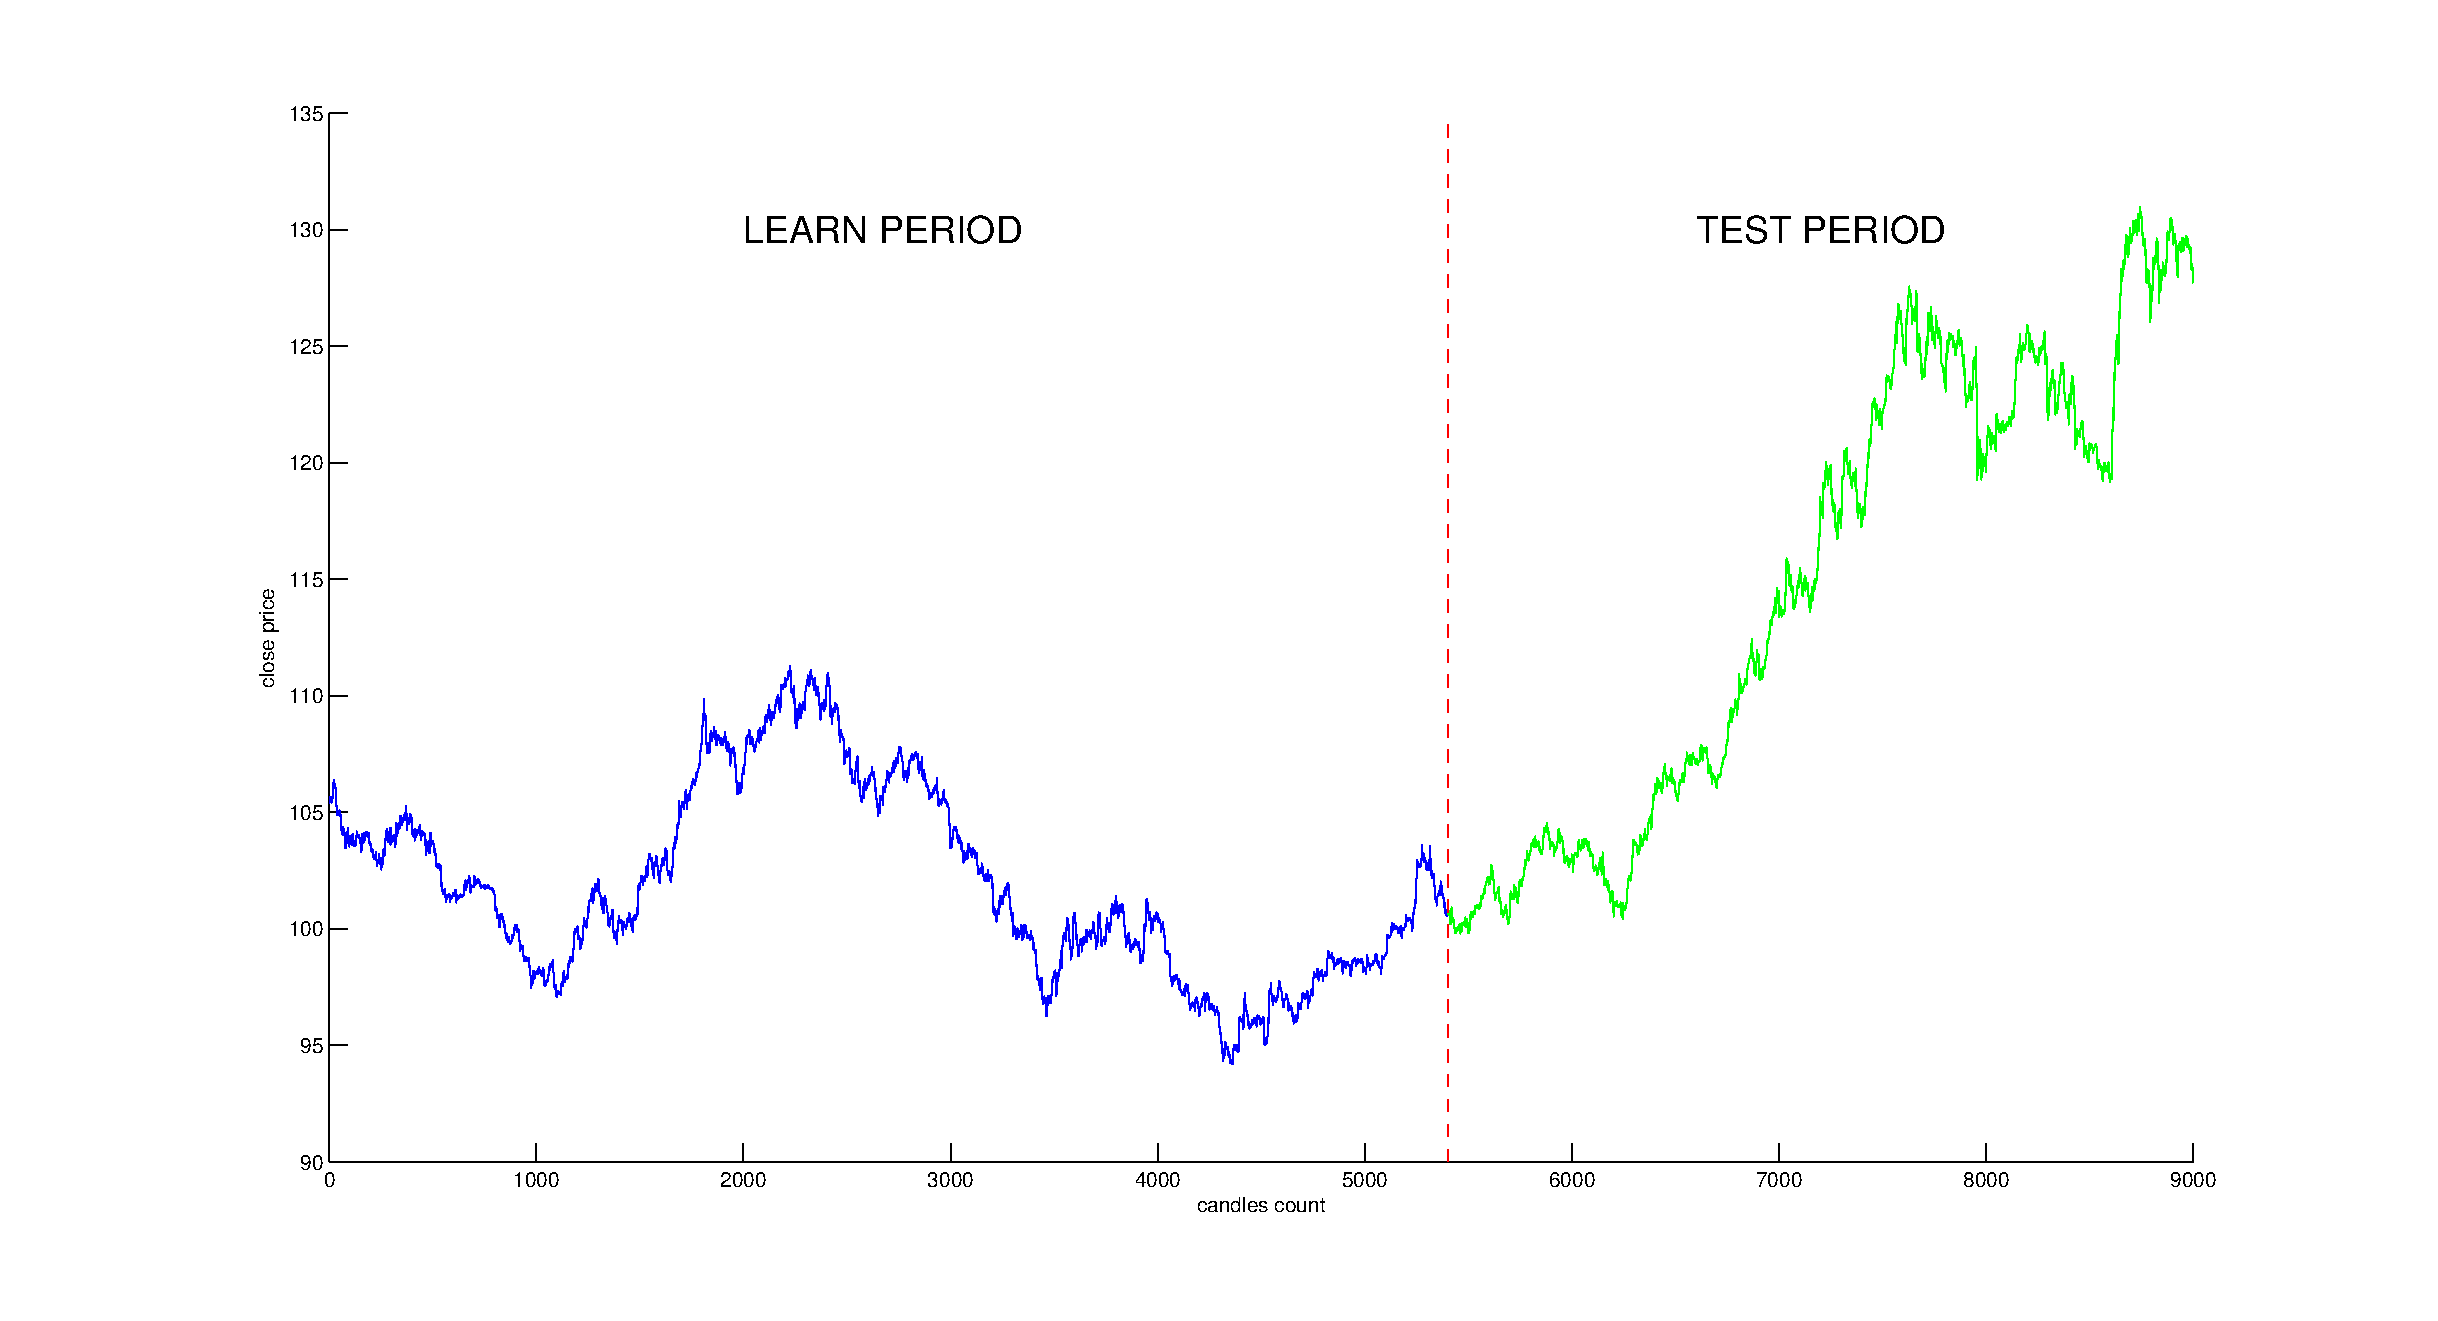
\includegraphics[width = \textwidth]{podzialDanych.eps}
\caption{Studied time series with the division into the learn and test part}
\label{rysunek2roc}
\end{figure}
\FloatBarrier
The entire data set (candles) is divided into two parts: the learn ($60 \%$ of the total) and test ($40\%$ of the total). During studies an optimal value for $k$ on a period of learning was searched, then verified obtained results for the test period. Selecting the optimal value of the parameter $ k $ was determined in two ways:
\begin{itemize}
\item the resulting final profit,
\item Calmar ratio.
\end{itemize}
\newpage
\noindent \textbf{I The results of maximizing the profit.}\\
\begin{figure}[h!]
\centering
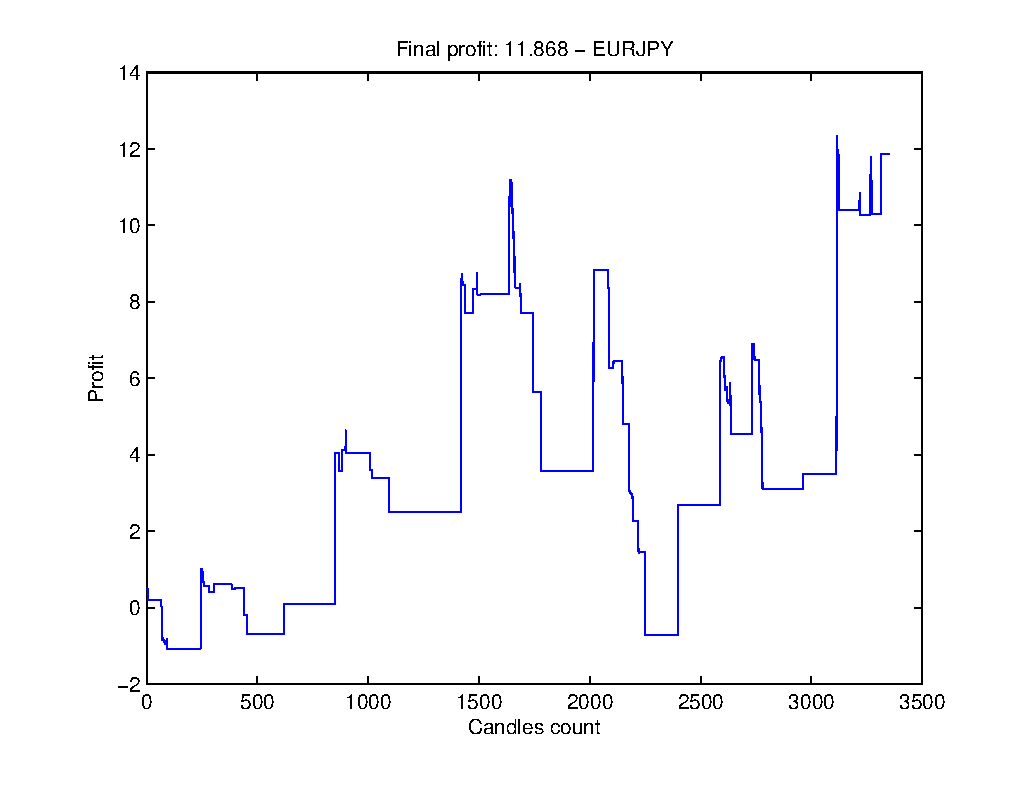
\includegraphics[width = 0.7\textwidth]{ROC_EURJPY_LS_SearchBestK_zysk.eps}
\caption{Cumulative return for the test period of EURJPY  while maximizing the profit}
\end{figure}
\FloatBarrier
\begin{verbatim}
LEARN PERIOD
The length of the cycle: 	89
Cumulative return: 	16.81
Calmar ratio: 	2.66
The number of opened long positions: 	100
The number of opened short positions:  	100

TEST PERIOD
The length of the cycle: 	89
Cumulative return: 	11.87
Calmar ratio: 	1.00
The number of opened long positions: 	61
The number of opened short positions: 	61
\end{verbatim}

\noindent \textbf{II The results of maximizing the Calmar ratio.}\\
\begin{figure}[h!]
\centering
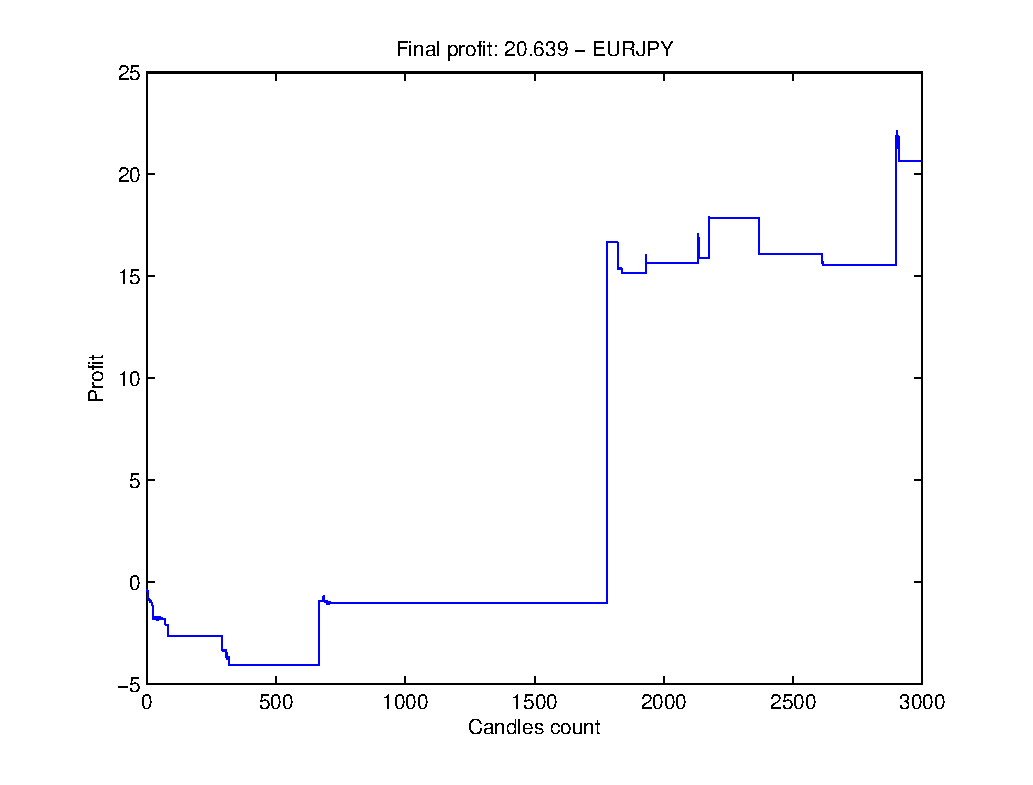
\includegraphics[width = 0.7\textwidth]{ROC_EURJPY_LS_SearchBestKCalmar_zysk.eps}
\caption{Cumulative return for the test period of EURJPY  while maximizing the Calmar ratio}
\end{figure}
\FloatBarrier
\begin{verbatim}
LEARN PERIOD
The length of the cycle: 	230
Cumulative return: 	12.82
Calmar ratio: 3.83
The number of opened long positions: 	52
The number of opened short positions:  	51

TEST PERIOD
The length of the cycle: 	230
Cumulative return: 	20.64
Calmar ratio: 	5.08
The number of opened long positions: 	28
The number of opened short positions: 	29
\end{verbatim}

